\section{Metode in rezultati} 

Nalogo smo razdelili na 2 dela: napovedovanje kota pogleda uporabnika, ter
napovedovanje optimalnih uporabljenih tokov glede na kote. Glede na takšno
delitev v tem poglavju tudi predstavimo našo rešitev. Začnemo pa z opisom
metode za preverjanje kvalitete napovedi.

\subsection{Interno prečno preverjanje}
Ker je bilo dovoljenih oddaj na lestvico le $10$, smo morali implementirati
interno prečno preverjanje \eng{Cross validation}. Le tako smo lahko namreč
učinkovito določili hiperparametre za uporabljene algoritme ter jih primerjali
med seboj.

Prečno preverjanje je v tem primeru delovalo tako, da smo nekaj tokov iz učne
množice odstranili iz nje ter jih razbili na odseke dolge po 8 sekund, pri
čemer smo za zadnje 4 sekunde odstranili kote. Pri rezanju tokov smo zaradi
količine podatkov dovolili tudi, da se izrezani tokovi prekrivajo.  Poleg tega
smo namesto računanja rezultata s formulo, ki je bila uporabljena za lestvico,
raje računali povprečno kvaliteto uporabnikovega pogleda.

\subsection{Napovedovanje kota pogleda}

Za napovedovanje kota pogleda smo preizkusili 3 različne strategije.

\subsubsection{Konstantni kot}
Prva strategija je temeljila na podatkih pridobljenih iz vročinskih slik
\ref{fig:heatmap}. Iz teh lahko vidimo, da uporabniki zelo radi gledajo
posnetek v okolici kota $0\degree$. Tako smo za vsak kot napovedali kar
konstantni kot, kjer je bila vsota stolpca vročinske slike največja. Iz slik
lahko še opazimo, da se optimalen konstantni kot spreminja glede na uporabljeno
okno, torej je izbira tega precej pomembna.

\subsubsection{Zadnji znani kot}
Druga strategija je temeljila na histogramu \ref{fig:rel}, iz
katerega lahko razberemo, da se pogledi uporabnikov večinoma ne spreminjajo
veliko skozi čas. Na podlagi tega je bila ideja, da je napovedovanje zadnjega
znanega kota pogleda uporabnika zelo dobra aproksimacija dejanskega pogleda za
naslednjih nekaj desetink sekunde.

\subsubsection{Seam Carving}
Navdih za zadnjo strategijo je prišel s strani fantastičnega algoritma
uporabljenega za skaliranje slik, pri čemer na sliki pomembnejši
deli ohranjajo pravo razmerje. Algoritem je originalno znan pod imenom
\textit{Seam Carving}\cite{seamcarving}, oziroma \textit{Content Aware Scaling}
v programskem orodju Photoshop. Deluje tako, da na sliki najprej vsakemu pikslu
določi `energijo' (npr. velikost gradienta), nato pa iz zgornje vrstice pikslov
na sliki poišče pot ki minimizira to energijo do spodnje, pri čemer se lahko
pomika iz posameznega piksla le v tri neposredno v vrstici pod njim. Nato to
pot preprosto izreže iz slike in ta postane tako za en piksel ožja.

Drugače povedano za naše potrebe lahko algoritem iz vsakega para $\left(\theta,
t\right)$ določi optimalno pot skozi video z začetkom v podanem paru ter koncem
v $t' = 60s$.

V naši verziji namesto energije tako uporabimo kar vročinsko sliko, ki smo jo
predstavili v \ref{fig:heatmap}, pri čemer smo mi zainteresirani v
maksimizaciji energije. Algoritem iskanja optimalne poti nato dejansko temelji
na zelo preprosti uporabi dinamičnega programiranja. Našo modificirano verzijo
lahko opišemo z naslednjo enačbo:
\begin{displaymath}
  sc(\theta, t) = heatmap(\theta, t) + \left\{ \begin{array}{ll}
                                            0 & \textrm{če $t = 60$,}\\
                                            \max\{mp(\theta'-\theta) \cdot sc(\theta', t+1)\}_{\theta' \in \theta + [-\alpha, \alpha]} & \textrm{sicer,}
  \end{array} \right.
\end{displaymath}

kjer so:
\begin{itemize}
  \item[-] $\theta \ldots$ aktualni kot,
  \item[-] $t \ldots$ aktualni čas,
  \item[-] $heatmap \ldots$ lookup tabela za izračunano vročinsko sliko (glej~\ref{fig:heatmap}),
  \item[-] $mp \ldots$ funkcija ki glede na relativni kot pove `verjetnost' premika (uporabljena kot utež premika), in
  \item[-] $\alpha \ldots$ parameter ki določa, koliko kotov na vsako stran preverimo.
\end{itemize}

Racionalizacija za uporabljeno vročinsko sliko je ista, kot je bila v opisu
prvega algoritma, podobno ideja za funkcijo $mp$ stoji za analizo histogramov
relativnih premikov uporabnikov (glej \ref{fig:rel}). S tem smo nekako
združili dobri ideji obeh prvih algoritmov v enega samega. Smo pa se morali
precej igrati z izbiro okna oz. parametrov. Naivna uporaba pravokotnega okna za
vročinske slike ter parametri ki zagotovijo čim boljše prileganje Gaussove
distribucije k dejanskim podatkom namreč niso dali najboljših rezultatov.

Na delovanje algoritma torej lahko vplivamo na nekaj načinov:
\begin{itemize}
  \item s spremembo uporabljenega okna pri izdelavi vročinske slike,
  \item s spremembo resolucije vročinske slike,
  \item s spremembo funkcije $mp$, ter
  \item s spreminjanjem parametra $\alpha$.
\end{itemize}

Na vse od teh parametrov smo gledali kot na hiperparametre ter iskali optimalne
vrednosti s pomočjo postopka opisanega v naslednjem podpoglavju.

\subsection{Ocenjevanje napovedanih kotov}
Ker za ocenjevanje kvalitete z uporabo implementiranega prečnega preverjanja
potrebujemo tudi tokove, smo kvaliteto napovedanih kotov interno preverjali
malce drugače. Podobno kot pri prečnem preverjanju smo izdelali učno in
validacijsko množico, vendar pa smo tokrat gledali povprečno $L1$ razdaljo
med napovedanim ter dejanskim kotom v zadnjih štirih sekundah tokov. Graf
\ref{fig:ang} prikazuje povprečno odstopanje v stopinjah v odvisnosti od
časa. Tu je lepo razvidno, da zadnja metoda dejansko rezultira v najpravilnejše
napovedi kotov.

\begin{figure}[H]
  \centering
  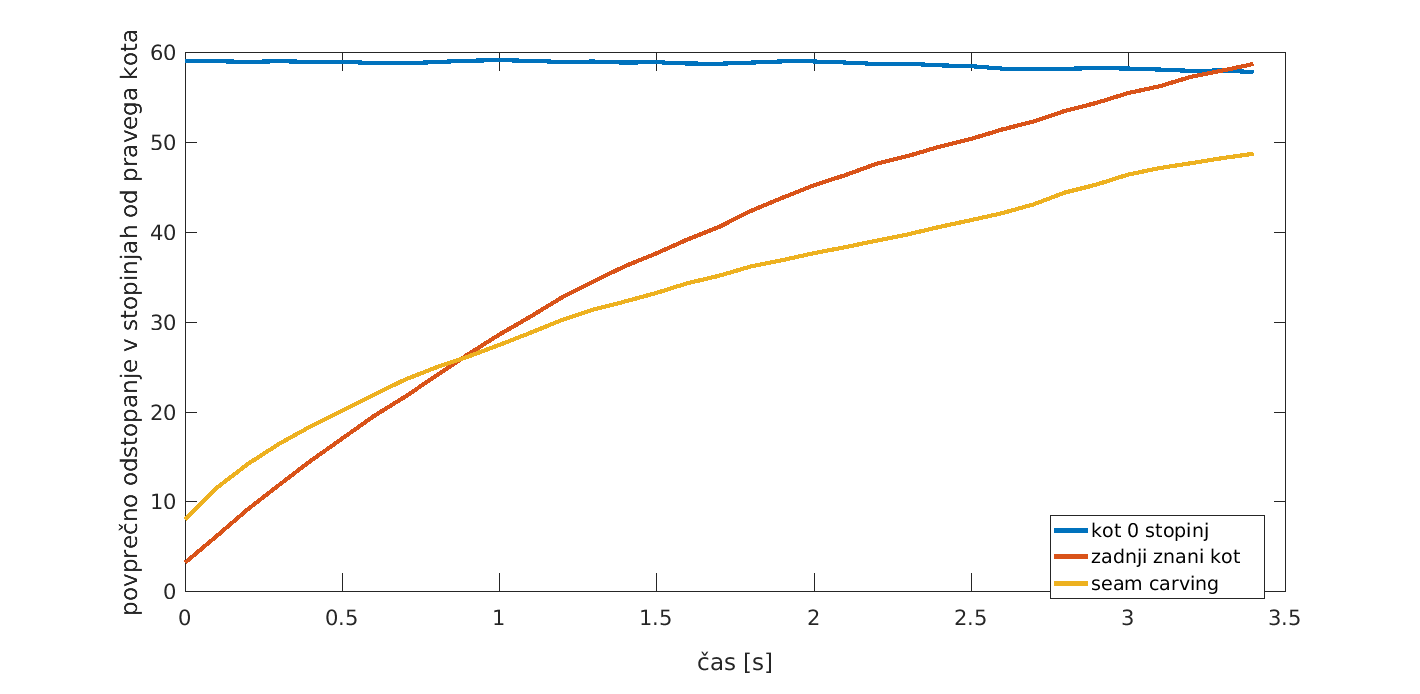
\includegraphics[width=300pt]{{img/ang}}
  \caption{Graf odstopanja napovedanega kota od dejanskega kota v odvisnosti od
  časa za različne metode.}
  \label{fig:ang}
\end{figure}

V našem primeru smo za zmagovalno rešitev torej uporabili algoritem, ki je
temeljil na tretji strategiji. Pri tem podatke najprej prevzorčili na časovno
resolucijo $1/10$ sekunde, ter kotno resolucijo $1\degree$. Za izdelavo
vročinske slike smo uporabili Welchovo okno, za dinamično programiranje pa smo
gledali kote 4 stopinje v vsako smer od trenutnega kota, z verjetnostjo premika
definirano kot Gaussova funkcija s povprečjem $0$ in standardnim odklonom
$\sqrt{80}$. Izgled poti, ki jih algoritem ubere je razviden is slike \ref{fig:pat}

\begin{figure}[H]
  \centering
  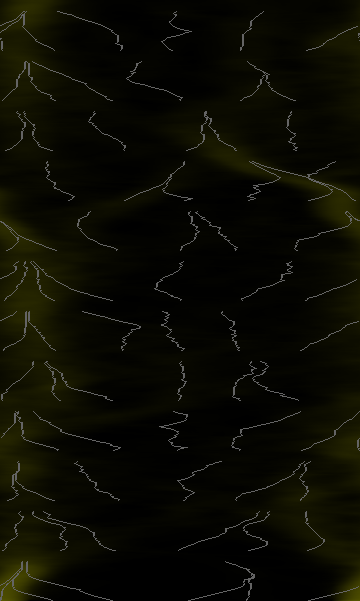
\includegraphics[width=110pt]{{img/paths}}
  \caption{Graf izbranih poti končnega algoritma. Z belo barvo so izrisane poti
  na vročinski sliki.}
  \label{fig:pat}
\end{figure}

\subsection{Napovedovanje optimalnih uporabljenih tokov}
Drugi del naloge je predstavljala specifikacija največ 100 tokov. Tu smo
izhajali iz ideje, da želimo za podane kote pri prvih $4$ sekundah tokov
uporabniku zagotoviti optimalno izkušnjo: video kvalitete $100\%$ za celoten
pogled. Na podlagi tega smo izdelali 90 tokov kvalitete $100\%$ ter kotnega
razpona $4\degree$: $\left\{ \left(4\cdot\theta, 4\cdot\theta + 4 - 1,
100\%\right); \theta \in [0, 89] \right\}$, pri čemer smo lahko nato za vsak
kot izračunali optimalne tokove, ki so nam zagotovili čim večji razpon na obe
smeri (pri omejitvi, da ne presežemo skupne pasovne širine).

Ker pa na ta način ne pokrijemo vseh $360\degree$ pa smo si tu ustvarili še
pomožen ``dummy'' tok, ki je zgolj izpolnjeval zahtevo, da je kvaliteta na
vsakem od $360$ kotov vsaj ena stopinja: $\left(0, 359, 1\%\right)$.

Tokovi kvalitete $100\%$ lahko pokrijejo le kot $96\degree$ ($360$ pasovne
širine potrebujemo za dummy tok). Ker smo na sliki \ref{fig:ang} odkrili da
povprečno optimalen kot zgrešimo za precej več, smo tu poskusili tudi na
pameten način uporabljati tokove z več različnimi kvalitetami. Če bi namreč
uporabljeno kvaliteto postopoma zniževali bi lahko pokrili večji kot in tako ne
bi za napačne napovedi prejeli le ene točke. Vendar pa se je vsak poskus
nadgradnje uporabljene strategije izkazal za slabšega, tako da smo na koncu
uporabili kar opisanih $90$ $100\%$ tokov.
